\documentclass[twoside,twocolumn,9pt]{article}

\usepackage[super,sort&compress,comma]{natbib}
\usepackage[left=1.5cm, right=1.5cm, top=1.785cm,
bottom=2.0cm]{geometry}
\usepackage[english]{babel}
\usepackage[T1]{fontenc}
\usepackage{hyperref}
\usepackage{graphicx}
\graphicspath{{./figures}{../figures}}

%\usepackage{epstopdf}
\usepackage{epstopdf}
\author{Mateo Barria-Urenda, José Antonio Gárate}
\title{Thermodynamic characterization of the adsorption of amino acids
  onto pristine graphene and graphene oxide}
\date{}

\begin{document}

\maketitle

\abstract{}

\section{Introduction}

% Context

First synthesized in 2004 \cite{Novoselov_2004}, graphene has since
experienced an explosive growth in interest \cite{Randviir_2014}.  For
pristine graphene, it's interactions with other particles are mainly
due to Van der Waals forces and $\pi-\pi$ stacking. \cite{Zuo_2012} As
pristine graphene is chemically inert \cite{Eftekhari_2017} a
classical description of it is expected to suffice in simulations.
Multiple molecular dynamics studies on the interactions between
proteins and carbon based nanoparticles (CBNs) --such as graphene--
have been published \cite{Zheng_2003, Ge_2011, Zuo_2012, Chong_2015,
  Duan_2015, Shityakov_2015, Al_Qattan_2018,Puigpelat_2019,
  Gonz_lez_Durruthy_2020, Li_2020}

% Need

% Task

% Work


\section{Methods}

\subsection{Umbrella Sampling}

\subsection{Well Tempered Multiple Walk Metadynamics}

\subsection{Molecular Dynamics Simulation}

\begin{figure}[htbp]
\centerline{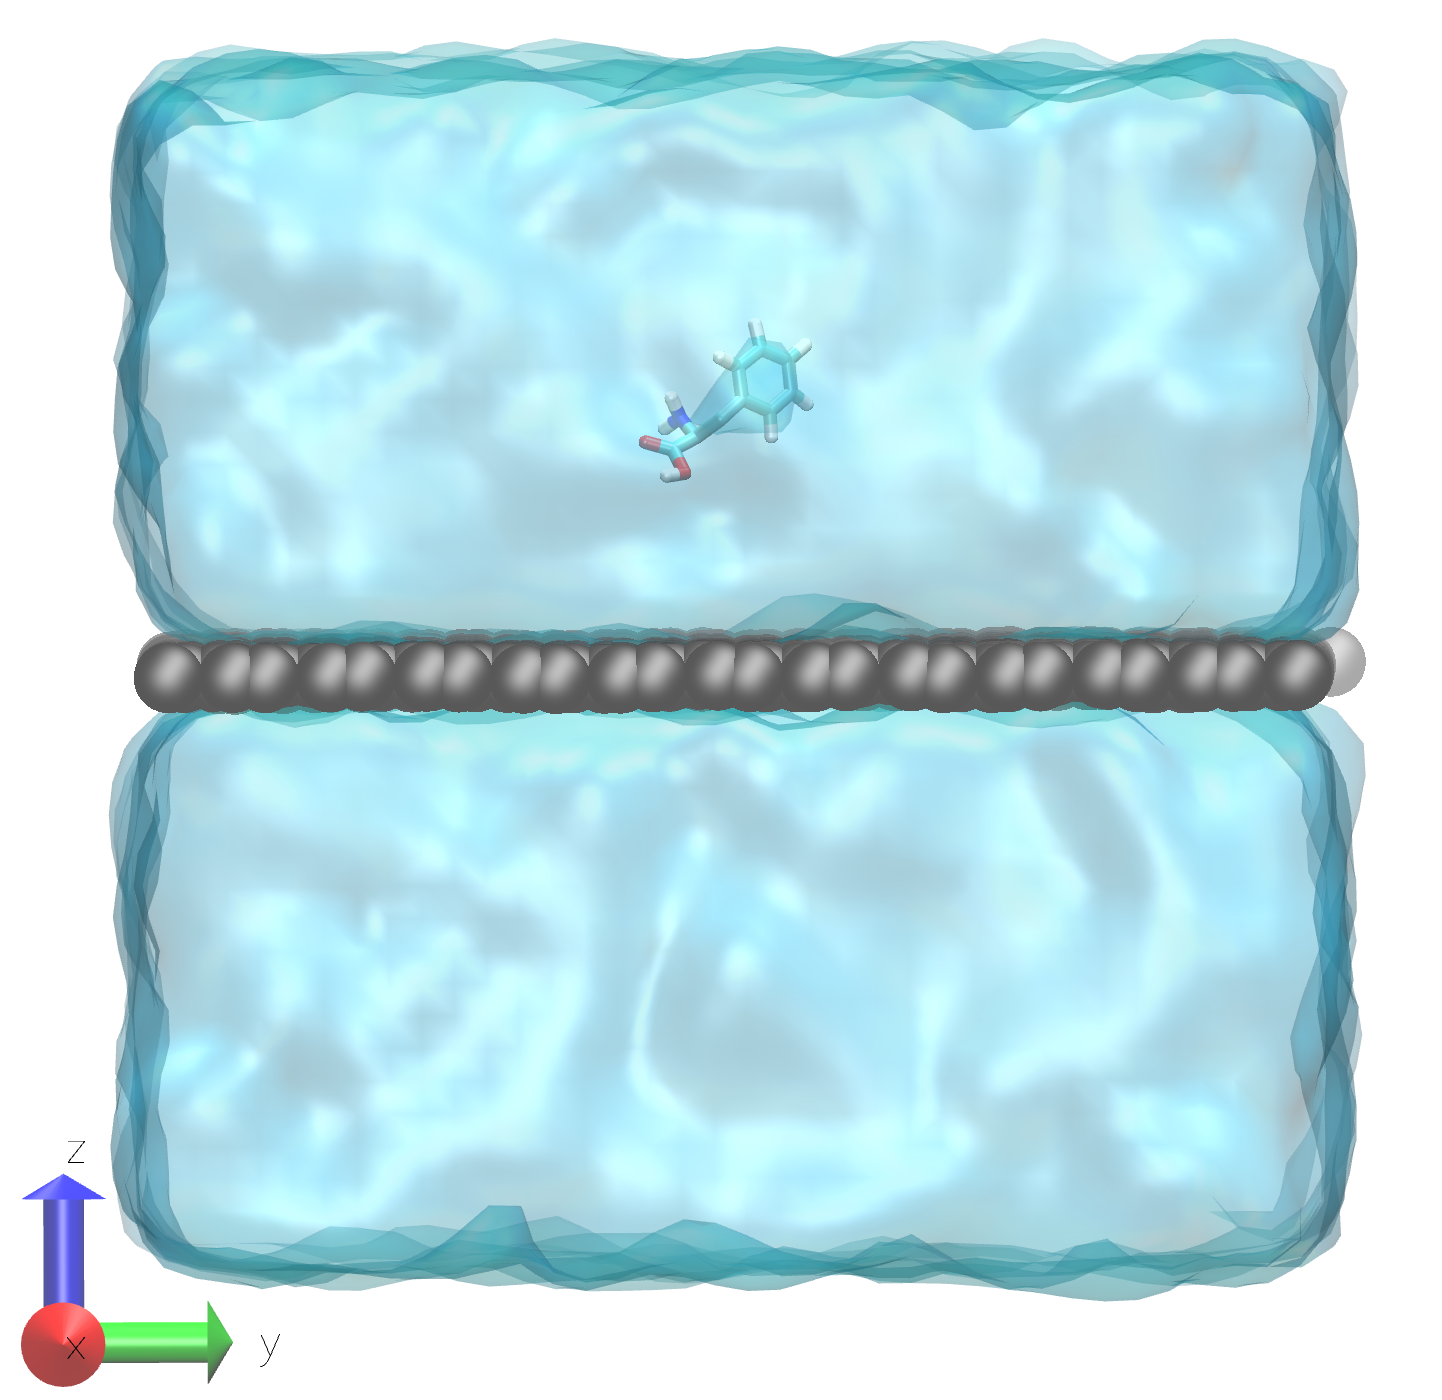
\includegraphics[width=\columnwidth]{/home/mbarria/Dropbox/Papers/graphene_adsorption_paper/figures/Pristine_System.png}}
\caption[]{\label{fig:system-pristine} Example of simulated pristine
  graphene systems. An amino acid (in this case Phenylalanine) above a
  graphene layer (in gray) inside a periodic water box.}
\end{figure}

\begin{figure}[htbp]
\centerline{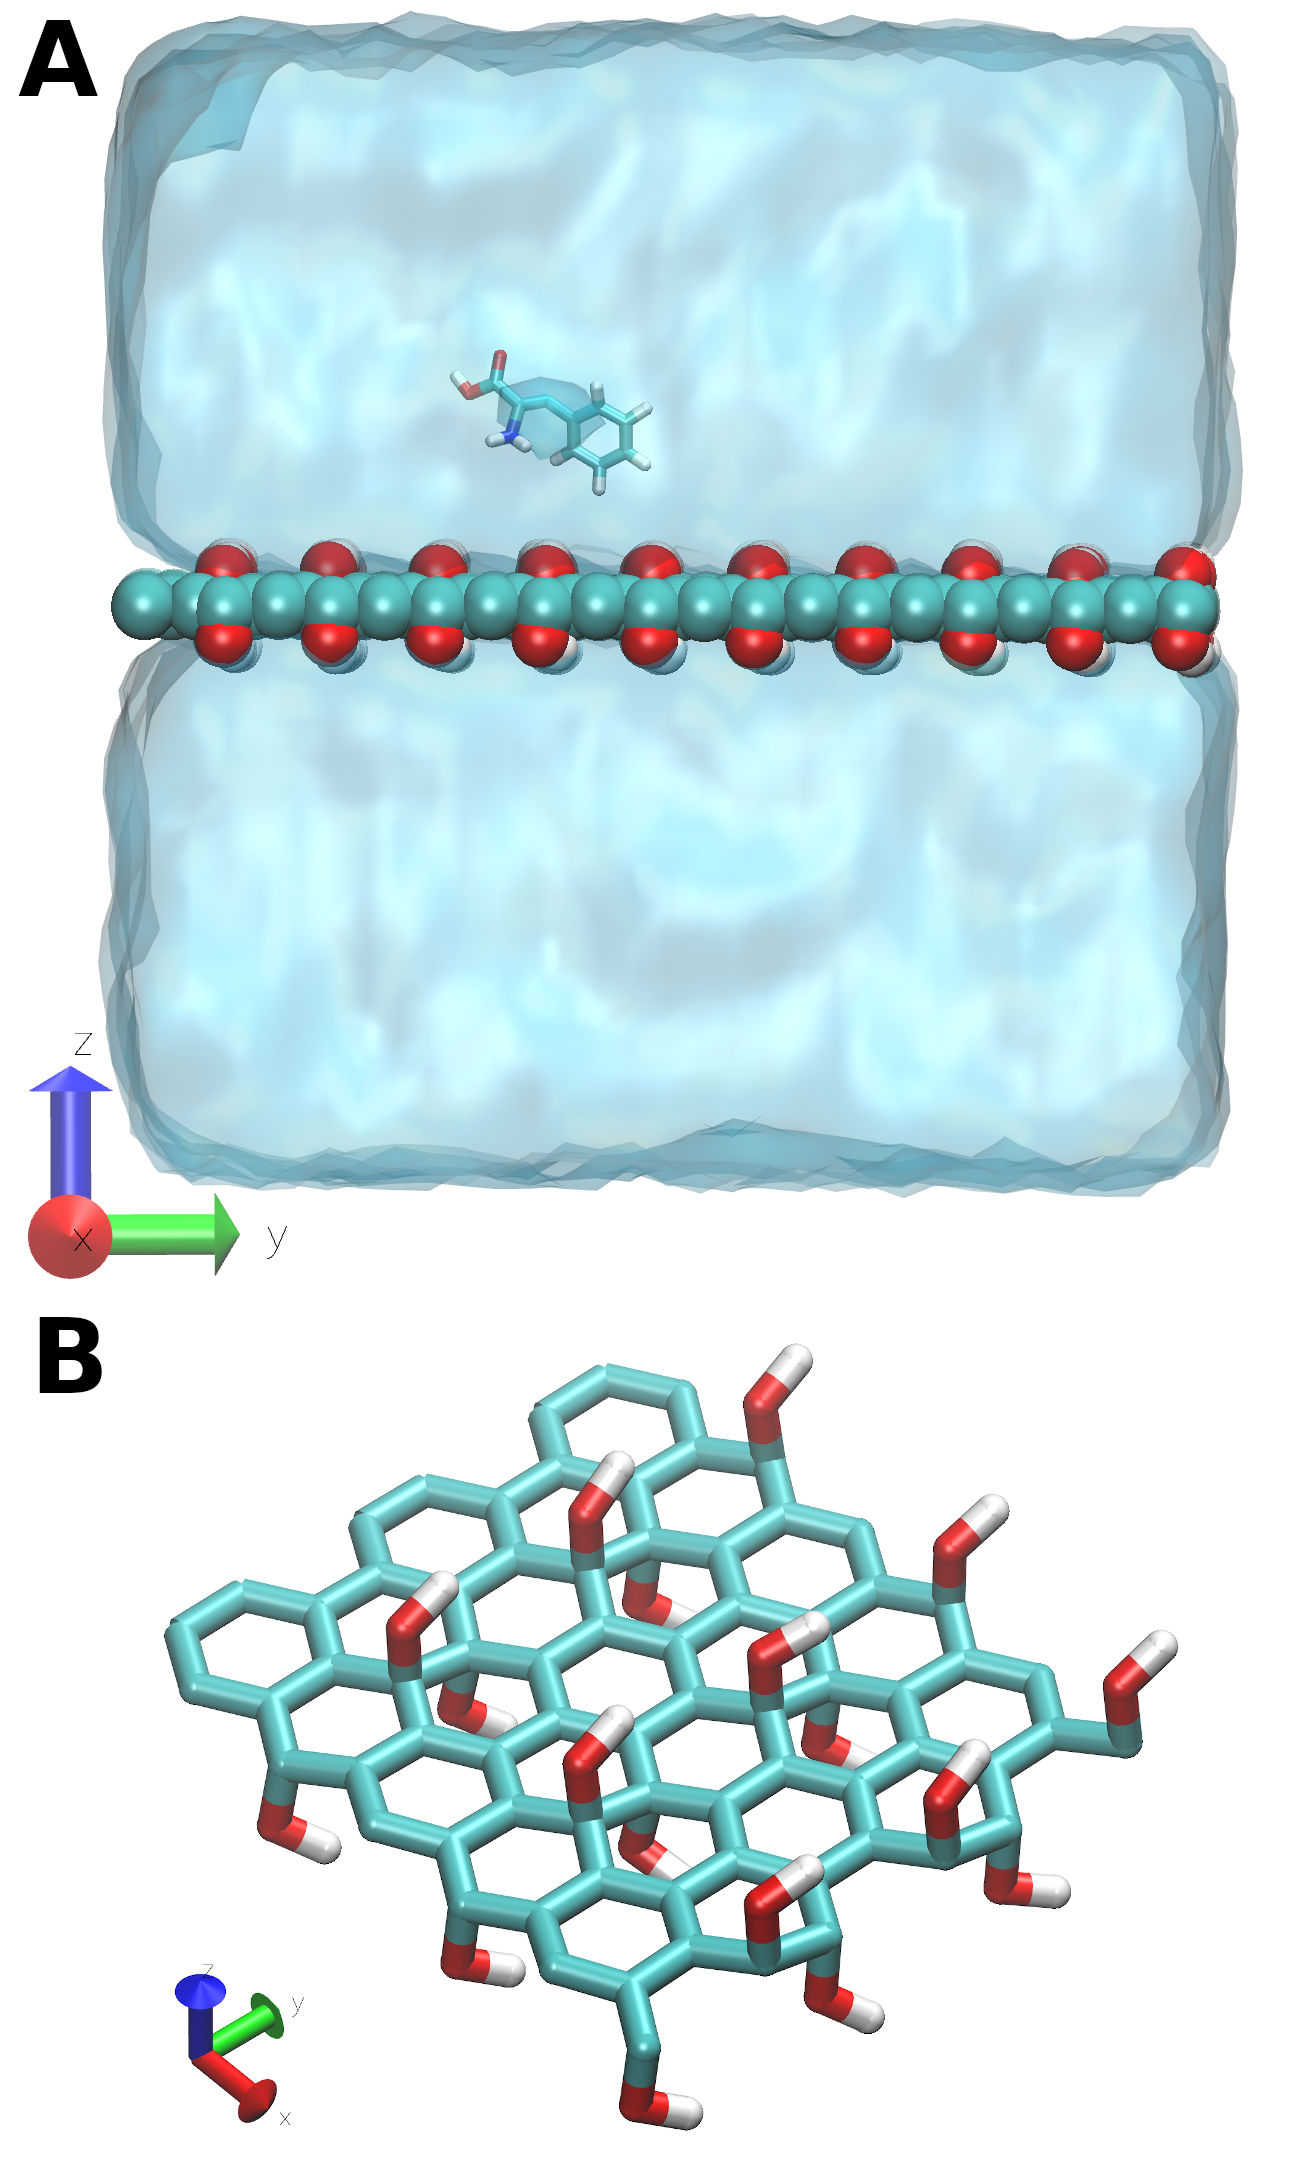
\includegraphics[width=\columnwidth]{/home/mbarria/Dropbox/Papers/graphene_adsorption_paper/figures/Oxidized_System_and_Unit.png}}
\caption[]{\label{fig:system-oxidized} a) Example of simulated oxidized
  graphene systems. An amino acid (in this case Phenylalanine) above a
  graphene layer (C in gray, O in red, H in white) inside a periodic
  water box. b) Segment of the oxidized graphene layer depicting the
  oxidation pattern. (C in gray, O in red, H in white)}
\end{figure}

\subsection{Quantum Mechanics / Molecular Mechanics}

\section{Results}

\begin{figure*}[htbp]
\centerline{\includegraphics[width=\textwidth]{/home/mbarria/Dropbox/Papers/graphene_adsorption_paper/figures/Differences_by_names_and_weight.png}}
\caption[]{\label{fig:differences} Differences of adsorption over a
  pristine graphene layer for free energies ($\Delta A_{ads}$),
  energies ($\Delta E_{ads}$) and entropies ($T \Delta S_{ads}$) for
  all proteinogenic amino acids. Top row (a, c, and e):
  $\Delta A_{ads}$, $\Delta E_{ads}$, and $T \Delta S_{ads}$, arranged
  by amino acid classification on the basis of side-chain
  interactions. Amino acids are labeled on the x-axis by their three
  letter code. Bottom row (b, d, and f): $\Delta A_{ads}$,
  $\Delta E_{ads}$, and $T \Delta S_{ads}$, as a function of molecular
  weight of the amino acid. Amino acids are labeled by their markers
  with their one letter code. In all cases amino acids are in a
  neutral state unless marked with a positive ($+$) or negative ($-$)
  sign.}

\end{figure*}

\begin{figure*}[htbp]
\centerline{\includegraphics[width=\textwidth]{/home/mbarria/Dropbox/Papers/graphene_adsorption_paper/figures/Differences_by_names_and_weight_25o.png}}
\caption[]{\label{fig:differences} Differences of adsorption over an
  oxidized graphene layer for free energies ($\Delta A_{ads}$),
  energies ($\Delta E_{ads}$) and entropies ($T \Delta S_{ads}$) for
  select amino acids. All values are relative to Glycine's, which is
  set to 0. Top row (a, c, and e): $\Delta A_{ads}$,
  $\Delta E_{ads}$, and $T \Delta S_{ads}$, arranged by amino acid
  classification on the basis of side-chain interactions. Amino acids
  are labeled on the x-axis by their three letter code. Bottom row (b,
  d, and f): $\Delta A_{ads}$, $\Delta E_{ads}$, and
  $T \Delta S_{ads}$, as a function of molecular weight of the amino
  acid. Amino acids are labeled by their markers with their one letter
  code. In all cases amino acids are in a neutral state unless marked
  with a positive ($+$) or negative ($-$) sign.}

\end{figure*}

\subsection{Adsorption Free Energy}

\subsection{Adsorption Entropy}

\subsection{Adsorption Energy}

\subsection{Diffusion}

\section{Conclusions}


\section*{Acknowledgements}
This work was partially supported by grant no. ICM-Economia grant
no. P09-022-F Centro Interdisciplinario de Neurociencia de Valparaiso,
Universidad de Valparaiso; FONDECYT 1180987 (to J.A.G.), PAI grant
no. 77170045 (to J.A.G.) and a doctoral scholarship from
CONICYT--PFCHA/DOCTORADO BECAS NACIONAL/2020--21201020.  Access to the
supercomputing infrastructure of the National Laboratory for
High-Performance Computing was supported through grant no. ECM-02
(Powered@NLHPC).


\bibliography{refs.bib}
\bibliographystyle{plainnat}

\end{document}

%%%Local Variables:
%%% mode: latex
%%% TeX-master: t
%%% End:
